\documentclass[conference, 11pt]{sty/IEEEtran}
% \documentclass[paper=a4, fontsize=11pt]{scrartcl}

\title{Secure Pairing}
\author{Erik Boss \and Max Hovens \and Anton Jongsma \and Aram Verstegen}
\date{\today}

\usepackage{hyperref}
\usepackage{amsmath, amssymb}
\usepackage{caption}
\usepackage{subcaption}
\usepackage{sty/mathtools}

\newlength{\arrow}
\settowidth{\arrow}{\scriptsize$100000000000$}
\newcommand*{\rarrow}[1]{\xrightarrow{\mathmakebox[\arrow]{#1}}}
\newcommand*{\larrow}[1]{\xleftarrow{\mathmakebox[\arrow]{#1}}}

\begin{document}

\maketitle

\begin{abstract}

In the world of mobile devices there is often no means of an established trust authority with which to establish a secure channel.
Therefore, there is ongoing research into methods for establishing a secure channel using ad hoc methods, so called \textit{secure pairing methods}.
Over the years, several techniques have been proposed to solve this problem.
In particular, such solutions require the use and availability of out-of-band channels.
In this paper we survey and assess a range of different techniques for establishing a secure pairing between devices.
These include protocols that do not require a specific out-of-band channel and also techniques for using specific out-of-band channels.
Furthermore, we create a proof-of-concept implementation for a technique that uses the displaying and reading of QR codes as an out-of-band channel.

\end{abstract}

\section{Introduction}
\label{sec:introduction}

The proliferation of electronic devices, mobile and otherwise, communicating over wireless channels leads to the problem of establishing a secure connection between the devices.
In particular, wireless channels can be eavesdropped and also manipulated with relative ease, making man-in-the-middle (MitM) attacks a relevant threat~\cite{kumar2009comparative}.
To eliminate the threat of MitM attacks, one would wish to establish a secure wireless channel.
This is where \emph{secure device pairing} comes in.

Secure device pairing, secure pairing for short, is the process of creating a secure channel between two devices that have no previous security context.
That is, a secure pairing scheme needs to be able to provide mutual authentication without relying on external trust anchors.
Because we cannot rely on an external infrastructure as a basis of trust most of the standard techniques are not easily applicable.
In particular, there is an need~\cite{kumar2009comparative} to do some part of the communication over an auxiliary channel, so-called out-of-band (OOB) channels.
These OOB channels have special security properties by virtue of the media over which the data travels~\cite{balfanz2002talking}.
They may, due to their nature, prevent MitM attacks by providing what is essentially a secure channel.
Devices can use these methods to agree upon keys out-of-band before communication takes place in-band, or to validate the key agreed upon in-band was not tampered with by a third party.
Note that we cannot just use the OOB channel for all our communication, we still need in-band communication over the wireless channel.
This is because OOB channels typically have very low bandwidth.
Which makes it important for performance reasons that communication over the OOB channel is used sparingly.

These OOB channels are managed by the users themselves and typically rely on human interaction to authenticate the communication over the wireless channel.
Suppose we use human visual capabilities as an OOB channel, for instance in the case of asking a user to compare images.
This channel is very hard to interfere with for an attacker without the human user(s) noticing, thus exhibiting one of these special security properties we mentioned.
Overall, there are many such OOB channels, some of which we shall discuss in subsequent sections in the paper.
One problem with such channels is that they often rely on a certain common set of interfaces.
However, interface-wise almost no two devices are alike and it is common for two very different devices to need a secure communication channel.
For instance, a recent mobile phone might have a (virtual) keyboard, a camera and a number of other sensors.
A simple wireless Bluetooth headset, however, likely has almost none of these things and is probably limited to just communicating over a wireless channel.
This makes establishing an OOB channel between such different devices challenging since we lack common interfaces.

There are two elements to a secure pairing scheme.
Essentially, we can often separate the content of the communication and the method of communication.
The content is determined primarily by the protocol, the method entails the way in which certain interfaces are used in order to use this protocol.
Most of our focus will be on the latter, since the protocols are typically not very elaborate.
We will mention, however, some of the common protocols used for establishing a secure pairing.

We structure our paper as follows.
We start off with a survey of the protocols and techniques used in secure device pairing.
In \autoref{sec:cryptographic_protocols_for_secure_device_pairing} we discuss a number of protocols used for secure device pairing, i.e., they specify the content of the communication.
These, as a rule, do not rely on a particular OOB channel.
Then, in \autoref{sec:secure_device_pairing_methods}, we discuss several methods of establishing a secure pairing.
We then proceed in \autoref{sec:assessment_of_the_state_of_the_art} to briefly assess the state-of-the-art in secure device pairing from both a security and a usability perspective.
Furthermore, we discuss an implementation of a secure device pairing system between two mobile phones relying on QR-codes as an OOB channel.
This serves as a case study and a convenient platform for discussing the security and usability of such systems, in particular the trade-offs between those two concepts.

\section{Cryptographic protocols for secure device pairing}
\label{sec:cryptographic_protocols_for_secure_device_pairing}

In this section we discuss two general ways of accomplishing the mutual authentication of two devices assuming a suitable OOB channel is in place.
These protocols determine the content of the information being exchanged without relying too much on the particular channel.
Note, however, that this does not mean that every, or even most, of the techniques described in the next section use one of these protocols.
Many of those exploit, or are limited by, the particular characteristics of their respective representations and/or OOB channels.
That said, these protocols are useful for achieving mutual authentication in a general way assuming the OOB is suitably capable.
The particular choice of protocols that we discuss seems representative of the group of secure pairing protocols using OOB channels.
At least in the sense that our research did not yield protocols that were significantly different to the ones chosen.

\subsection{Talking to Strangers}
\label{ssec:talking_to_strangers}

A technique dating back to 2002, \emph{Talking to Strangers}~\cite{balfanz2002talking} is a system that relies on a suitable OOB channel in order to transmit pre-authentication data after which standard authentication protocols can be implemented.
A suitable OOB channel in this system must have the following two properties:

\begin{itemize}
    \item Support demonstrative identification.
        This entails the identification of a specific object, or a set of objects, based on their physical context.
        For instance, the pointing of an infra-red laser at an object in order to single out that particular object for communication.
    \item Authenticity.
        This entails the fact that an attacker must find it infeasible to transmit on the particular OOB channel, at least without said transmission being detected by legitimate users.
\end{itemize}

Note that we do not need the data transmitted over the OOB channel to be secret, we only need it to be authentic.

\emph{Talking to Strangers} uses such a suitable OOB channel for achieving mutual authentication by means of public-key encryption (PKE).
The problem of achieving mutual authentication when one has authenticated copies of each other's public keys is actually very simple.
This means that we only need to get authenticated copies of the public keys, which is where the OOB channel comes into play.
Specifically, each party sends their public key over the normal wireless channel and a hash of said public key over the OOB channel.
The hash serves as a \emph{commit} on the public key.
After this pre-authentication step, any number of normal authentication protocols can be executed as long as they can make use such authenticated public keys.

More formally, the pre-authentication looks as follows:
Given addresses $addr_A$ and $addr_B$ for parties $A$ and $B$, their respective public keys $pk_A$ and $pk_B$ and a collision resistant hash function $h$, we execute the following protocol over the OOB channel:

\begin{enumerate}
    \item $A \rightarrow B: addr_A, h(pk_A)$
    \item $B \rightarrow A: addr_B, h(pk_B)$
\end{enumerate}

After which we can proceed with a standard key exchange protocol (e.g., SSL/TLS), the goal of which is typically to get an agreement on some shared (symmetric) key.
The particulars of such a key exchange protocol we shall not discuss as we consider it to be outside the scope of this paper.
Do note that this can be done over the wireless channel.
This works because we have committed in a secure way on the public keys we will be using.

\subsection{Short Authenticated Strings}
\label{ssec:short_authenticated_strings}

A \emph{Short Authenticated Strings} (SAS) protocol achieves mutual authentication, much like the previously discussed protocol.
The SAS protocol primarily utilizes a commitment scheme in order to get an agreement on each other's public keys in combination with an OOB channel for transmitting a short string.
This string is authenticated due to the nature of a suitable OOB channel, hence the name SAS.

A simple yet robust protocol using this technique is proposed in~\cite{pasini2006sas}, which we reproduced in \autoref{fig:sas}.
It works by having two parties, say A and B, pick a random value and having A commit on this value.
Party B then sends its random value in the clear to A.
When this is done, A sends B its decommit value after which B opens the commit, revealing A's random value.
Now both parties have each other's random value but they are not sure whether these values are correct.
Since all communication so far has been on the wireless channel, an attacker might have been able to tamper with the messages so far.
To fix this, both parties compute the XOR of the random values they received and subsequently send the other party this XOR'ed value over the OOB channel.
Both parties then just check whether the values are the same.

\begin{figure*}
    \centering
\[
\begin{array}{c c c}
    \text{A} & & \text{B}  \\
    \text{input}: m_A & & \text{input}: m_b \\ \\ \hline \\
    R_A \in_U \{0,1\}^k & & R_B \in_U \{0,1\}^k \\
    (c,d) \gets commit(m_A, R_A) & \rarrow{c} & \\
                                 & \larrow{R_B} & \\
                                 & \rarrow{d} & \hat{R}_A \gets open(m_B, \hat{c}, \hat{d}) \\
    SAS \gets R_A \oplus \hat{R}_B & \rarrow{auth_{A}(SAS)} & SAS =^? \hat{R}_A \oplus R_B \\
    \text{check SAS is the same} & \larrow{auth_{B}(SAS)} & \\ 
\end{array}
\]
With: \\
$(c,d) \gets commit(m,r)$ generates commit value $c$ and decommit value $d$ for a key $r$ with tag $m$; \\
$r \gets open(m,c,d)$ yields $r$ if $(c,d)$ is a possible output for $commit(m,r)$; \\
$auth_{ID}(m)$ a message $m$ over an authenticated (OOB) channel from $ID$;
$m_A = m_B$ in an honest run of the protocol.
\caption{SAS protocol for mutual authentication}
\label{fig:sas}
\end{figure*}

This is arguably one of the simpler SAS protocols.
It assumes that their is a bidirectional OOB channel between the two devices.
\cite{saxena2008automated} and~\cite{saxena2006secure} propose very similar protocols that can be executed using unidirectional OOB channel.
However, these have slightly weaker security guarantees~\cite{saxena2008automated}.

\section{Secure device pairing methods}
\label{sec:secure_device_pairing_methods}

In this section we describe several pairing methods proposed in the literature.
We can distinguish different kinds of secure pairing methods.
Mostly, they differ in the amount of human interaction necessary and the OOB channels they use.
Some require only some preliminary setup from the user, others require the user to participate and others do not require user intervention at all.
The OOB channels can vary, but some manifestation of the visual channel seems to be the most popular choice.

\subsection{Image comparison}
An early approach to the problem of secure pairing involves image comparison.
On both devices an image of the OOB data is shown and the user is asked to compare both images.
The underlying protocol is the one described in \autoref{ssec:talking_to_strangers}.
Examples are \textit{Snowflake}~\cite{goldberg1996visual}, \textit{Random Arts Visual Hash}~\cite{perrig1999hash} and \textit{Colorful Flag}~\cite{dohrmann2002public}.
These methods require both devices to have a display with a reasonable resolution, making it impractical for devices like bluetooth headsets, but very suitable for modern mobile phones.

\subsection{Seeing is Believing}
In Seeing-is-Believing (SiB)~\cite{mccune2005seeing} camera phones are used to set up a pairing between two devices.
Given at least one device with a camera we can make sure that this device is communicating with the device we look at through the camera.
The device with a camera takes a snapshot of the barcode encoding of relevant cryptographic data, for instance the data in one of the protocols in \autoref{sec:cryptographic_protocols_for_secure_device_pairing}.
The cryptographic data is then used to bootstrap a secure connection between the two devices.

This method can work with a number of different sets of interfaces.
Ideally we have two devices, each of which has a camera \emph{and} a display.
% Since both devices have displays we can manage authentication with either displaying a long-term public key or an ephemeral one (by randomizing the displayed information) an.
We could do mutual authentication in a general way by applying, for instance, the \emph{Talking to Strangers} technique.
However, we can also manage with less than that.
If only one device has a camera we need to affix a barcode containing the necessary cryptographic information (e.g., a long-term public key or a commitment thereof) to the device.
In this case we can still authenticate the camera 
There are a few more combinations of interfaces to be examined and for the sake of comprehensiveness we shall reproduce in \autoref{table:sib} the full table of combinations of interfaces as found in~\cite{mccune2005seeing}.

\begin{table}[h]
    \begin{tabular}{ c | c c c c }
      X/Y  & CD & C & D & N \\ \hline
        CD & $\checkmark$ & $\checkmark^*$ & $\checkmark$ & $\checkmark^*$ \\
        C & $\checkmark$ & $\checkmark^*$ & $\checkmark$ & $\checkmark^*$ \\
        D & presence & presence & X & X \\
        N & x & x & x & x \\
    \end{tabular}
    \\ \\
    \small{Check whether X can authenticate to Y, C = camera, D = display, CD = both, N = neither, $\checkmark$ = strong authentication possible, $\checkmark^*$ = affixed barcode necessary, presence = can only verify the presence of a device, X = no authentication possible.}
    \caption{Authentication capabilities}.
    \label{table:sib}
\end{table}

Of course, we need both sides to be able to authenticate to do mutual authentication, i.e., the CD - CD combination.

\subsection{VIC}
\label{ssec:vic}

VIC~\cite{saxena2006secure}, or Visual authentication based on Integrity Checking, is meant as an successor of SiB, which we saw in the last section.
Recall that we noted that mutual authentication is only possible in SiB when both devices are equipped with cameras and displays (see \autoref{table:sib}).
In VIC we achieve mutual authentication even in the cases where SiB could only give one \emph{presence}.
However, we do need an additional step of user interaction.
VIC works as follows, where $h$ is a hash function and $K_A, K_B$ are A's and B's public keys respectively:

\begin{enumerate}
    \item $A \rightarrow B: K_A$
    \item $B \rightarrow A: K_B$
    \item $A: h_A \gets h(K_A \| K_B)$
    \item $B: h_B \gets h(K_A \| K_B)$
    \item $A \rightarrow B(\text{visual}): h_A$
    \item $B$: compare $h_A$ and $h_B$, if they match $B$ indicates acceptance to the user, reject and abort otherwise.
    \item $A$: prompt the user as to whether $B$ accepted or not. $A$ accepts if the user indicated that $B$ accepted, reject and abort otherwise.
\end{enumerate}

It is not hard to see that indeed this provides mutual authentication even in the camera-display scenario.
The intuition is that we only need one unidirectional visual channel if we use the user as a third party that relays to party A whether party B accepted or not.
The result of which is that we can get mutual authentication, like in SiB, with less interfaces than SiB due to SiB needing a bidirectional visual channel.

% TODO: de zin hierboven herschrijven, ref naar orig paper?

% In this method one device uses its camera to take a snapshot of a barcode encoding of, for example, the public key of the other device.
% The minimum set of interfaces for this approach to work is one device with a display, and one with a camera, making it again unsuitable for low-end devices.

\subsection{Blinking lights}
Related to \textit{Seeing is Believing} and VIC is the \textit{Blinking lights}~\cite{saxena2006secure} method.
Instead of a display and a camera the devices in the method use a LED and a light-sensor or camera.
The LED-equipped device transmits the authentication data by blinking the LED.
The other device recovers the data by recording the blinking and looking at the gaps between distinct blinks.
The actual protocol is the same as in \autoref{ssec:vic}.

In \emph{Blinking Lights} we represent a short gap between blinks as a '0' and long gaps as '1', the complete authentication data is then just a bitstring of binary representations of these gaps.
Since we cannot know when a receiver starts receiving the transmitter has to repeat the message over and over.
Indeed, the fact that we only have a unidirectional channel (LED to camera) does not allow to indicate that the receiver started receiving.
Moreover, we cannot know at which point in the transmitted data we start receiving.
This requires the receiver to accept any of the bit rotations of the expected value.
So for the expected bitstring $n$ we accept $n$ possible bitstrings.

\subsection{Shake well before use}
A different approach is taken in \cite{mayrhofer2009shake}, where two devices are supposed to be shaken together in one hand to do the pairing.
Eavesdropping this particular OOB really seems almost impossible, making this an interesting proposal.
Also, shaking is a very distinctive gesture, making it relatively easy to derive measurements that can be mapped to bitstrings.
It matches features extracted from the sensor data to derive a cryptographic key.

It is also noted that while the shaking has sufficient entropy to be useful in key generation, its primary use is in key verification.
That is, similar to the SAS protocol in \autoref{ssec:short_authenticated_strings} it may be more useful to just send random bytes to each other and \emph{then} verify that was done correctly by means of an OOB channel, in this case the shaking gesture.

The feature extraction is a process that involves corrections for time alignment and spatial alignment before the data is usable at all.
Indeed, it is easy to see that the particular way one holds both devices before shaking can lead to somewhat different measurements in each device.
In particular, the time alignment is done through segmentation and the spatial alignment through normalization.

\subsection{Loud and Clear}
\label{ssec:loud_and_clear}

Loud and Clear (LaC)~\cite{goodrich2006loud} is a technique that uses audio as an OOB channel.
The underlying protocol is the same as in \autoref{ssec:talking_to_strangers}, although there is also a version that uses a SAS protocol like in \autoref{ssec:short_authenticated_strings}~\cite{kumar2009comparative}.
It works by vocalizing, using a specialized text-to-speech engine, authentication strings into syntactically correct English sentences.

Two modes are possible, speaker-speaker mode and speaker-display mode.
They require the user to respectively compare two vocalized strings or compare the vocalized string with a textual representation of such a string.
Consider, for instance, the check that occurs in the pre-authentication for \emph{Talking with Strangers}.
We need to check whether the $pk_A$ that $A$ sent to $B$ is the correct one.
We can use LaC to have $A$ vocalize its $pk_A$ and have $B$ do the same, the user simply compares and either accepts or rejects.

\subsection{HAPADEP}
\label{ssec:hapadep}

Similar to Loud-and-Clear, HAPADEP~\cite{soriente2008hapadep} utilizes sound in order to get a pairing.
Its intended use is in situations where one may not have an available wireless connection.
It can use the audio channel for all messages instead.
That said, it can also be used in such a way that only some messages are sent using this audio channel, everything else can go via wireless.

For transmitting any message in general over the audio channel, a special codec is applied to the message and output the result over the speaker.
The receiver then decodes whatever it gets on its microphone back to the original message.
Protocol-wise it uses a system that is very similar to LaC.
First the respective public keys are sent over the audio channel by encoding the key to audio, outputting it over the speaker and decoding it back to its original form on the receiver's end.
Then the public keys are vocalized on both devices, similiar to LaC, to verify the keyexchange was done correctly.
The user verifies that these two vocalized keys, or hashes of keys, are indeed the same.

\subsection{Graphical passwords}
\label{ssec:graphical_passwords}

Graphical passwords are somewhat different from the previous methods.
As the name implies it entails the entering of passwords in a graphical manner as opposed to the usual practice of entering PINs or alphanumeric passwords in general.
The idea is that these graphical passwords can provide a similar level of security while being more memorable.
Note that these techniques do not necessarily use an OOB channel, they really are passwords in the more traditional sense, which is really what sets them apart from some of the other techniques discussed in this paper.
However, we can use them in the same way we use PINs for secure pairing, i.e., create a (temporary) password on one device and enter the password on the other device.
In a sense this uses the human memory as an OOB channel.

In \cite{schaub2013exploring} five different types of graphical passwords are discussed: \emph{Pass-Go}, \emph{UYI}, \emph{TAPI}, \emph{CCP} and \emph{MIBA}.
As an addition you might consider the Android gesture swipe unlocking scheme as a more recent example of such a system.
However, that particular scheme suffers from problems in terms of predictability of patterns, lack of possibilities, easy shoulder surfing and even smudge attacks~\cite{aviv2010smudge}.
The five techniques mentioned in \cite{schaub2013exploring} seem to cover quite a few different types of graphical passwords and we shall reproduce some of the descriptions with their respective characteristics here.

\subsubsection{Pass-Go}
\label{sssec:pass_go}

Pass-Go~\cite{tao2008pass} entails the drawing of dots and lines on a $n$-by-$n$ grid.
The grid can be colored in such a way that the user is being given hints pertaining to the correct password.
The size of $n$ primarily decides the security of the password, although $n$ does not really have to be very large.
$n = 5$ was suggested for phones but since screen sizes have increased we believe that this can be increased proportionally.
Also, the security can be enhanced by coloring the lines and dots differently.

\subsubsection{UYI}
\label{sssec:uyi}

UYI~\cite{hayashi2008use} is a scheme where the user has to pick a picture out of a number of distinct pictures.
This is done several times in succession.
The pictures are presented in a somewhat abstracted version such that the user that set the key can recognize the picture, but it makes it more difficult for an adversary.
The amount of challenges and the amount of options determine the security of this scheme.
Furthermore there must be a very large set of pictures to choose from.


\subsubsection{TAPI}
\label{sssec:tapi}

TAPI~\cite{citty2010tapi} is very similar to a regular PIN entry setup.
It consists of a grid of 16 icons where each icon is split into four parts, this essentially gives you a PIN number pad with 64 possibilities as opposed to just ten.

\subsubsection{CCP}
\label{sssec:ccp}

CCP~\cite{chiasson2007graphical} entails presenting the user with subsequent pictures where the user must click on a certain point in the picture.
Depending on the particular point being clicked on we get a different subsequent picture.
The password then is just a sequence of pictures with their respective correct click points.
If the user clicks on the wrong point a different image is presented than expected and thus this serves as a kind of feedback to the user.

\subsubsection{MIBA}
\label{sssec:miba}

MIBA~\cite{ritter2013miba} is a recent scheme that is very similar to CCP but with the addition of several new features.
It has a grid overlay to help the user with selecting click points.
Also, the differentiation between long and short presses on a given point can lead to different passwords in this scheme which aids in improving the password space.

\subsubsection{Password strength}
\label{sssec:password_strength}

\begin{table*}[t]
    \centering
    \normalsize{
    \begin{tabular}{c c c c c}
        Scheme & Rounds (14 bit) & Clicks (14 bit) & Rounds (42 bit) & Clicks (42 bit) \\
        \hline
        Pass-Go & 1 & stroke length 2 & 1 & stroke length 6 \\
        UYI & 3 & 3 & 10 & 10 \\
        TAPI & 3 & 3 & 7 & 7 \\
        CCP & 3 & 3 & 9 & 9 \\
        MIBA & 1 & 1-2 & 3 & 3-6 \\
        PIN & 1 & 4 & 1 & 13 \\
    \end{tabular}
    }
    \label{fig:pw}
    \caption{Password strength of graphical passwords}
\end{table*}

In order to fully appreciate the relative password strenghts of the different graphical password techniques described in this section we will reproduce the work done in~\cite{schaub2013exploring} in 
%\autoref{fig:pw}.
Table 1.

Note that all graphical passwords have a theoretical lower amount of user interaction in the form of clicks than a PIN of the same strength.
However, these calculations are based upon the theoretical password space, not a practical one and thus in practice these values may need adjusting.

\section{Assessment of the state-of-the-art}
\label{sec:assessment_of_the_state_of_the_art}
In this section we summarize our assessments of the classification, security and usability of different pairing methods.

\subsection{Classification}
A fine-grained classification of pairing methods is available in the research literature~\cite{chong2012usability}, but these considerations are mostly contextual and to a large extent outside the scope of our specific interests of usability and security.
We can broadly classify the pairing methods into the categories \emph{human-assisted channel}, \emph{device-controlled channel} and \emph{sensor synchronisation}, as categorised in \autoref{table:classification}.
In the cases where humans assist in forming the channel we can further divide between \textit{compare \& confirm} and \textit{compare \& select} approaches.

% table squishing
%\hspace{-3em}
%\begin{footnotesize}
\begin{table}[h]
    \centering
    \normalsize{
\begin{tabular}{c|c|c|c}
	Technique & HAC & DCC & SS \\
	\hline
	Image comparison & \checkmark &  & \\
	  Seeing is Believing &  & \checkmark &   \\
	   VIC & & \checkmark  & \\
	   Blinking Lights & \checkmark &  & \\
	Shake well before use &  &  & \checkmark \\
	       Loud and Clear & \checkmark & \checkmark & \\
    	  Graphical passwords & \checkmark &  &  \\
	 HAPADEP &  & \checkmark & \checkmark \\
	Infrared &  & \checkmark &  \\
\end{tabular}
    }
    \label{fig:classification}
    \caption{Classification of pairing methods by attributes `human-assisted', `device-controlled' and `sensor synchronization'}
\end{table}
%\end{footnotesize}
%\hspace{3em}

\subsection{Security assessment}
\label{ssec:security_assessment}

It makes little sense to evaluate the security of device pairing methods out of context: different devices make use of different communication channels, some of which are inherently harder to secure against eavesdropping.
As a cost consideration it is often unfeasible to add more communication channels to provide an out-of-band channel for more secure pairing: the topic is in fact characterised by elegant solutions to the pairing problem by using communication channels that already exist in the devices.

The assessment of what is secure is therefore based on the attacker model.
Secure pairing methods using an out-of-band channel try to defend against a Man-in-the-middle (MITM) attack, whereby an observer may actively or passively intercept (or possibly relay and modify) the communication between devices, which would defeat the desired goal of establishing a secure channel between two users who otherwise trust each other and their devices.
An eavesdropper intruding into the devices involved or compromising either of the users of the devices in the pairing is outside of the attacker model.

The risk of eavesdropping can be quantified in terms of the leakage to outside observers of the communication channels used.
In the case of device-controlled pairing with a high bandwidth channel we can employ cryptographic primitives to mitigate such leakage.
As a last resort, we can attempt to make interception of leaking signals very hard by raising the complexity and frequency of signals.
This is a property that we found difficult to quantify using formal methods in cryptography.
In all cases we prefer minimal leakage within a certain physical radius from the devices.

A final metric to consider in the context of security is the robustness of the OOB channel against Denial-of-Service (DoS) attacks, in other words, their availability.

Our considerations for these assessments are as follows, and are summarized in \autoref{table:security_properties}:
\begin{itemize}
	\item Image comparison is vulnerable to the same kind of observation, but the observed information may only be used in the same session and is thus not usable for a replay attack.
	The images can be auto-generated from shared secrets, to let users do verification of cryptographic keys established in-band to mitigate this leakage.
	\item Observing a Seeing is Believing pairing may similarly reveal the secret information that is communicated. A device-controlled pairing, such as also happens with Visual authentication based on Integrity Checking pairing (VIC) can secure against this with cryptography and signal complexity.
	The communication could perhaps be disturbed by bad lighting conditions, like for example a strobe light, making it difficult for the camera's to adjust for light intensity.
	\item Blinking lights are vulnerable to eavesdropping by an observer, since the light emitted by LED diodes is very bright in a certain light spectrum band, which can be clearly observed at a distance.
	Infrared LEDs exhibit the same leakage problem to a worse degree.
	Conversely, when there are multiple light sources active in the same part of the \textit{visible} spectrum it becomes more difficult to observe at a distance which of them are on or off. This is not the case with infrared signals which are meant to be machine-readable.
	The signal may again be disturbed by extreme lighting conditions such as under a strobe light.
	\item The shaking of two phones can incur subtle high-frequency signals to the accelerometers of the mobile devices, which is hard to observe without having access to the accelerometer data of a device that went through the same shaking pattern.
	Using a high-speed camera or similar visual observation of the pairing process does not reveal these subtle signals to an observer.
	We can use the signals to do verification of shared secrets agreed upon in-band.
	\item Loud and clear makes itself audible to the user (provided they have normal hearing), and as such also to any eavesdroppers. A man-in-the-middle would need to overpower the original sender in volume, making such tampering evident. A noisy environment would prevent the method from being applied successfully. Because this is a common occurrence, we deem this a low resistance to DoS attacks.
	\item Graphical passwords may be observed by an outside attacker, the different methods within this category may be vulnerable to a straightforward replay attack while others may be randomized and require several observations before the entire secret is recovered.
	%This is a user-assisted channel often found on devices without usable input sensors like Bluetooth headsets.
	The method may also be used to verify shared secrets communicated in-band have not been tampered with.
	\item HAPADEP makes use of audio signals, and is therefore susceptible to eavesdropping by conventional surveillance methods. It's a device-controlled channel, so cryptographic primitives can be employed, as can signal complexity.
\end{itemize}

In conclusion, we propose the following metrics for security assessment: the estimated \emph{leakage} in terms of the radius at which the signals dissipate comparatively; the ability to use strong \emph{cryptographic primitives} over an out-of-band channel or if the method can be used to validate shared secrets agreed upon in-band; whether the \emph{complexity of the signal} can be practically raised to further thwart eavesdroppers; and finally, how \emph{robust} the channel is against DoS attacks.

% table squishing
\hspace{-2em}
\begin{table*}[t]
    \centering
    \normalsize{
\begin{tabular}{c|c|c|c|c}
	Technique & Leakage radius & Crypto & Signal complexity & Robustness \\
	\hline
	Image comparison & Medium & Yes & Medium & High\\
     Seeing is Believing & Low & Yes & High & Medium \\
		     VIC & Low & Yes & High & Medium\\
	 Blinking Lights & Medium & Yes & Low & High\\
	Shake well before use & Low & Yes & High & High \\
	       Loud and Clear & High & No & No & Low \\
      Graphical passwords & Medium & No & Medium & High \\
		 HAPADEP & Medium & Yes & High & Medium \\
	  Infrared & High & Yes & Low & Medium \\
\end{tabular}
}
    \caption{Classification of pairing methods by security properties}
    \label{table:security_properties}
\end{table*}
\hspace{2em}

Based on this classification, we summarily conclude that the two variants of \textit{Seeing is Believing} and \textit{Shake well before use} have the best overall security properties in terms of leakage, enabling of cryptography and signal complexity.

%Another factor at play in the security of pairing in practice is the length of the secret message that is agreed upon through the chosen channel, i.e. \emph{key length}.
%Since none of the techniques considered define a required minimal or maximal key length, this aspect does not relate to the pairing methods investigated.
%In effect, we are free to choose the strength of the used key independently of the chosen method of pairing.

\subsection{Usability assessment}
\label{ssec:usability_assessment}

\subsubsection{System Usability Scores (SUS)}
Prior research into the usability of the secure pairing methods found in the literature~\cite{kumar2009comparative} established the System Usability Score (SUS) for the considered pairing methods, as well as measuring the perceived security and the time and success rate to complete the task of pairing by observing a group of 22 test subjects interacting with test implementations in a controlled environment.
The results of this study show that of the methods considered in this summary, PIN and image comparison methods have the best scores in every category.
Blinking lights takes the longest time to complete, has a relatively low SUS score and the lowest task completion rate.
Shake well before use was not considered in this usability study.

Our intended method, Seeing is Believing, has a relatively high task completion rate but on average takes a long time to complete.
Its established SUS score is about 50\% and the perceived security is about 60\%.

\subsubsection{Rushing user}
In a similar study \cite{kobsa2009serial} some of the same authors establish the resistance of pairing methods against so-called \textit{rushing user} behaviour.
The authors also recognize the distinction between device-controlled and user-assisted channels for pairing and concluded that the user-assisted pairing methods are more susceptible to the \textit{rushing user} behavior.

\subsubsection{Security failures VS non-security failures}
Another source on usability assessment contrasts usability and security directly~\cite{kainda2009usability} by measuring the number of failed pairing attempts using user-assisted out-of-band channels for \textit{comparing} and then \textit{selecting} or \textit{confirming} OOB data using mnemonics like numbers, alphanumeric strings, words and sentences in natural language, images, melodies and combinations thereof.
They conclude that neither method is suitable for secure and usable human-assisted OOB channels, but that \textit{copying} the data provided good results in both aspects.
The article concludes expressing interest in another option: using barcodes.

\section{Design}
\label{sec:design}
In line with the deliverables of this project, we have drafted a proof of concept implementation of a Seeing is Believing (SiB) secure pairing solution for Android mobile devices.
The design makes use of 2D bar codes (specifically, QR codes) to transmit and receive information, using the open source \textit{android-quick-response-code}\cite{aqrc} and \textit{zxing}\cite{zxing} libries.
We display a QR code on the first device, and scan it on the second device, and the other way around.
This creates a channel with reasonably high bandwidth.
A QR code can contain up to 1264 ASCII characters, scanning a QR code typically takes a couple of seconds. 
This channel can be eavesdropped by anyone within visual range of the display of the device.
However, in our opinion it is very difficult to perform a MitM attack without the user(s) noticing, because the devices have to be quite close (around 10 to 50 cm) to eachother for the QR-code scanning to succeed.

Because of the reasonably high bandwidth and the aforementioned properties of the channel, we decided to implement a Diffie-Hellman key exchange to establish a shared secret. The Diffie-Hellman protocol is considered secure against eavesdroppers.
The resulting shared secret is then converted to a PIN-code which can be used to do a conventional PIN-based Bluetooth connection pairing.

Although the Bluetooth 2.0 specification defines the possibility to do a Bluetooth pairing using Out-of-Band data, the bluetooth API of Android does not support this for third-party applications. Android implements a version of SAS, where the user is asked to compare two 6-digit numbers shown by the devices.

\subsection{Overview}
\label{ssec:overview}
The main application allows users to configure their devices to either initiate or receive a pairing request.
In both cases the clients generate their half of a Diffie-Hellman key exchange.
Once the receiver is done it will switch to sender mode, and the initiator will switch to receiver mode after the user confirms by pressing a button.

The userinterface shown in figure \ref{figui} shows the steps involved in executing a succesfull key exchange.

\section{Conclusion}
\label{sec:conclusion}
The secure pairing methods presented in this paper all have different characteristics.
Because we sought to implement a prototype for modern mobile phones, we have choosen to adapt the Seeing is Believing method.
Displaying a QR code and scanning it with a camera can be done on any modern phone.

The QR code mechanism allows us to establish Diffie-Hellman keys with reasonable length. In our implementation we choose a 2048 bit modulus, which is still considered secure for the foreseeable future according to the recently updated research survey at \textit{keylength.com}\cite{keylengthdotcom}.

The implementation work does show that the method is usable in practice, and we can conclude mobile devices equipped to scan and display QR codes are enabled to do strong key negotiation using this out-of-band channel.

The SiB method we implemented is only a prototype, but it demonstrates that using QR codes a keyexchange with sufficient strong keys is feasible. Althought the implementation lacks integration with Bluetooth itself, we consider it practical and sufficiently fast.


\newpage

\begin{figure}
\centering
\begin{subfigure}{0.28\textwidth}
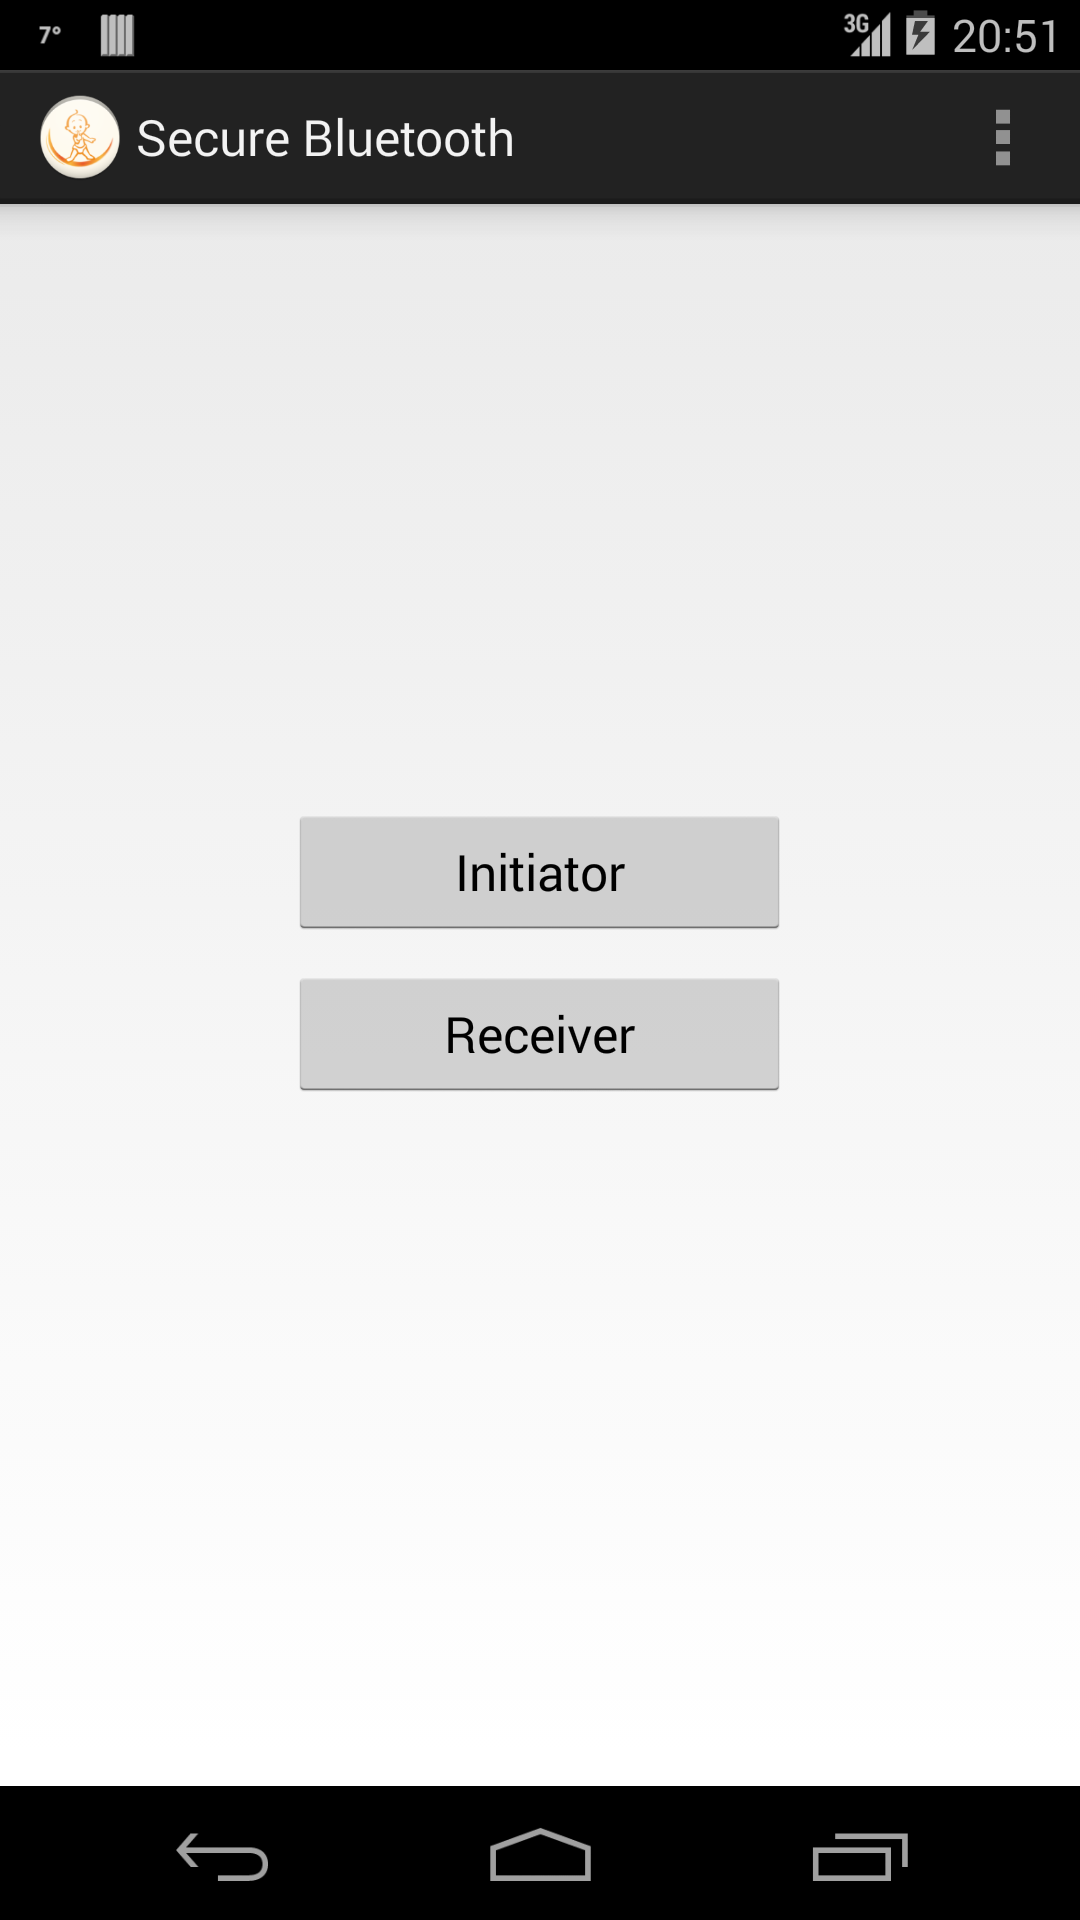
\includegraphics[width=\textwidth]{../screenshots/Screenshot_2013-12-01-20-51-28.png}
\caption{Select device role.}
\end{subfigure}

\begin{subfigure}{0.28\textwidth}
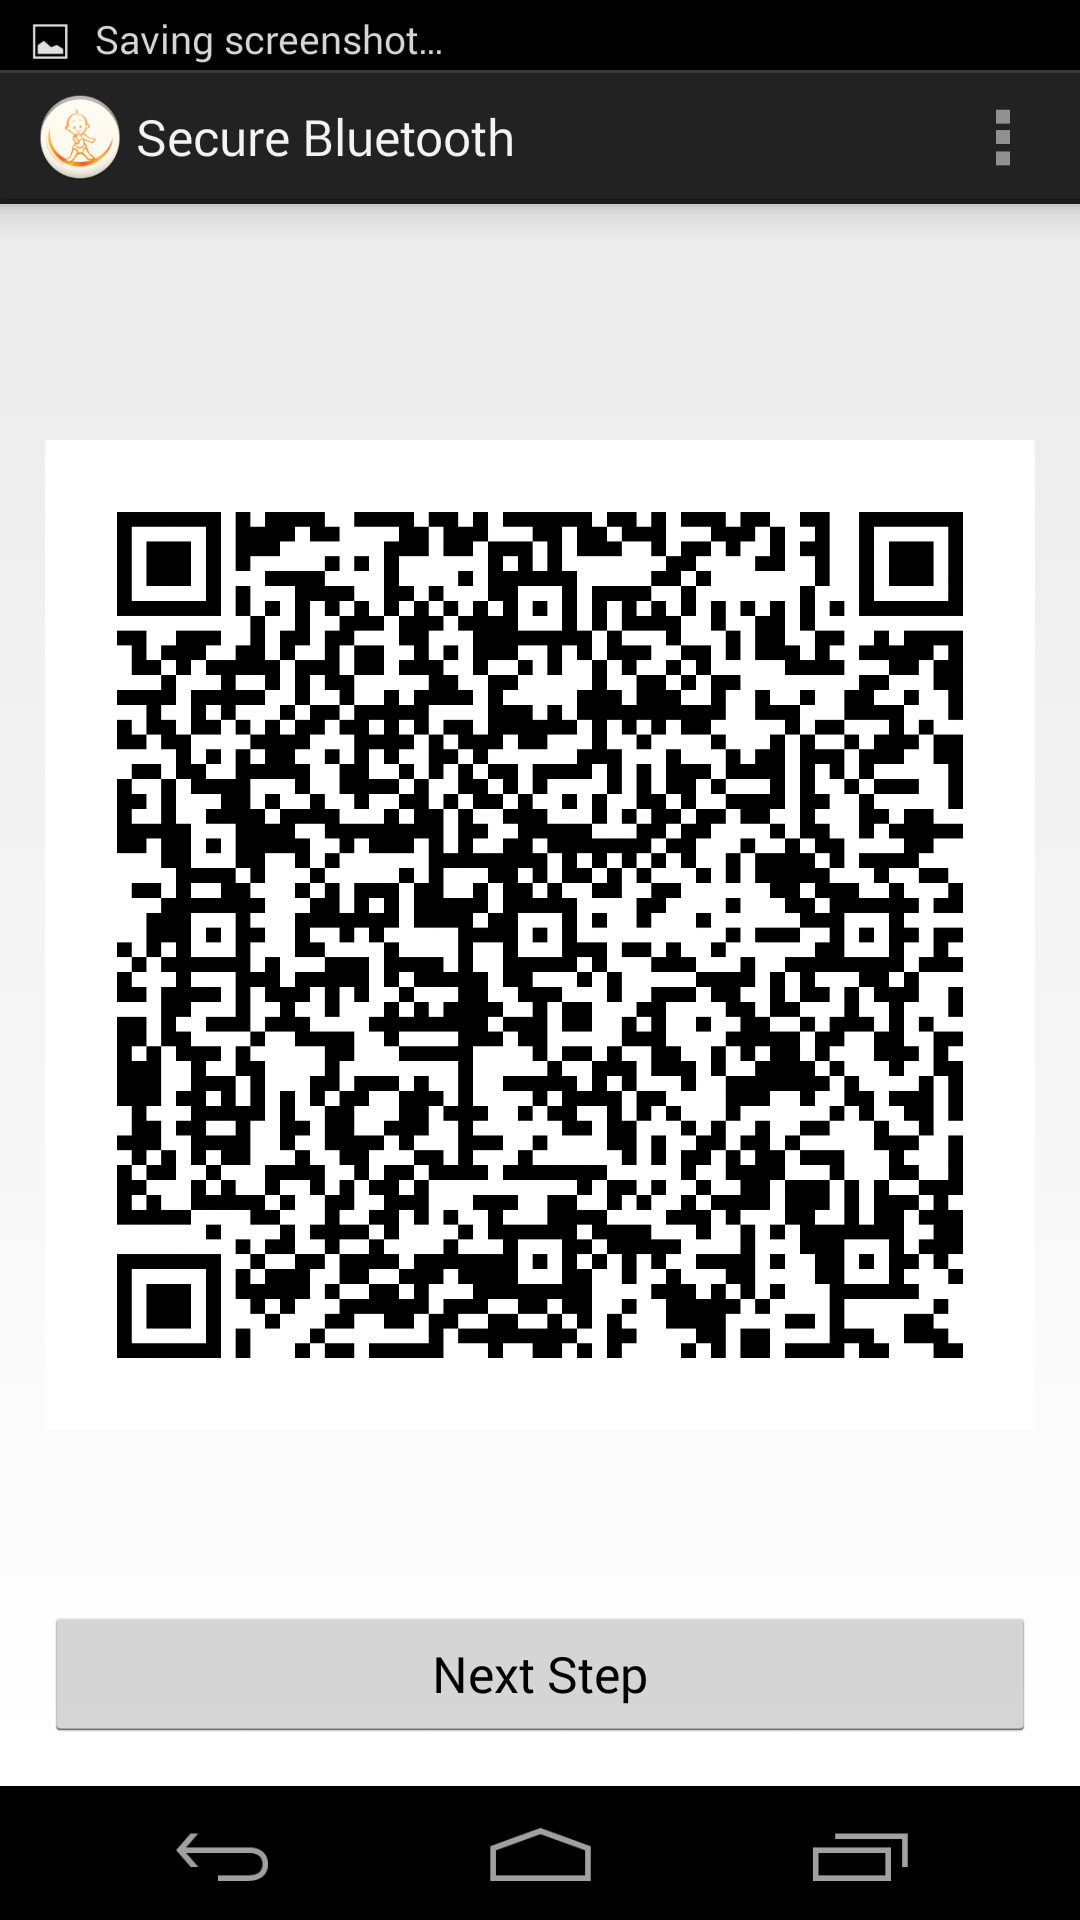
\includegraphics[width=\textwidth]{../screenshots/Screenshot_2013-12-01-20-51-32.png}
\caption{Initiating a DH key exchange via QR codes. Press next to switch roles.}
\end{subfigure}

\begin{subfigure}{0.28\textwidth}
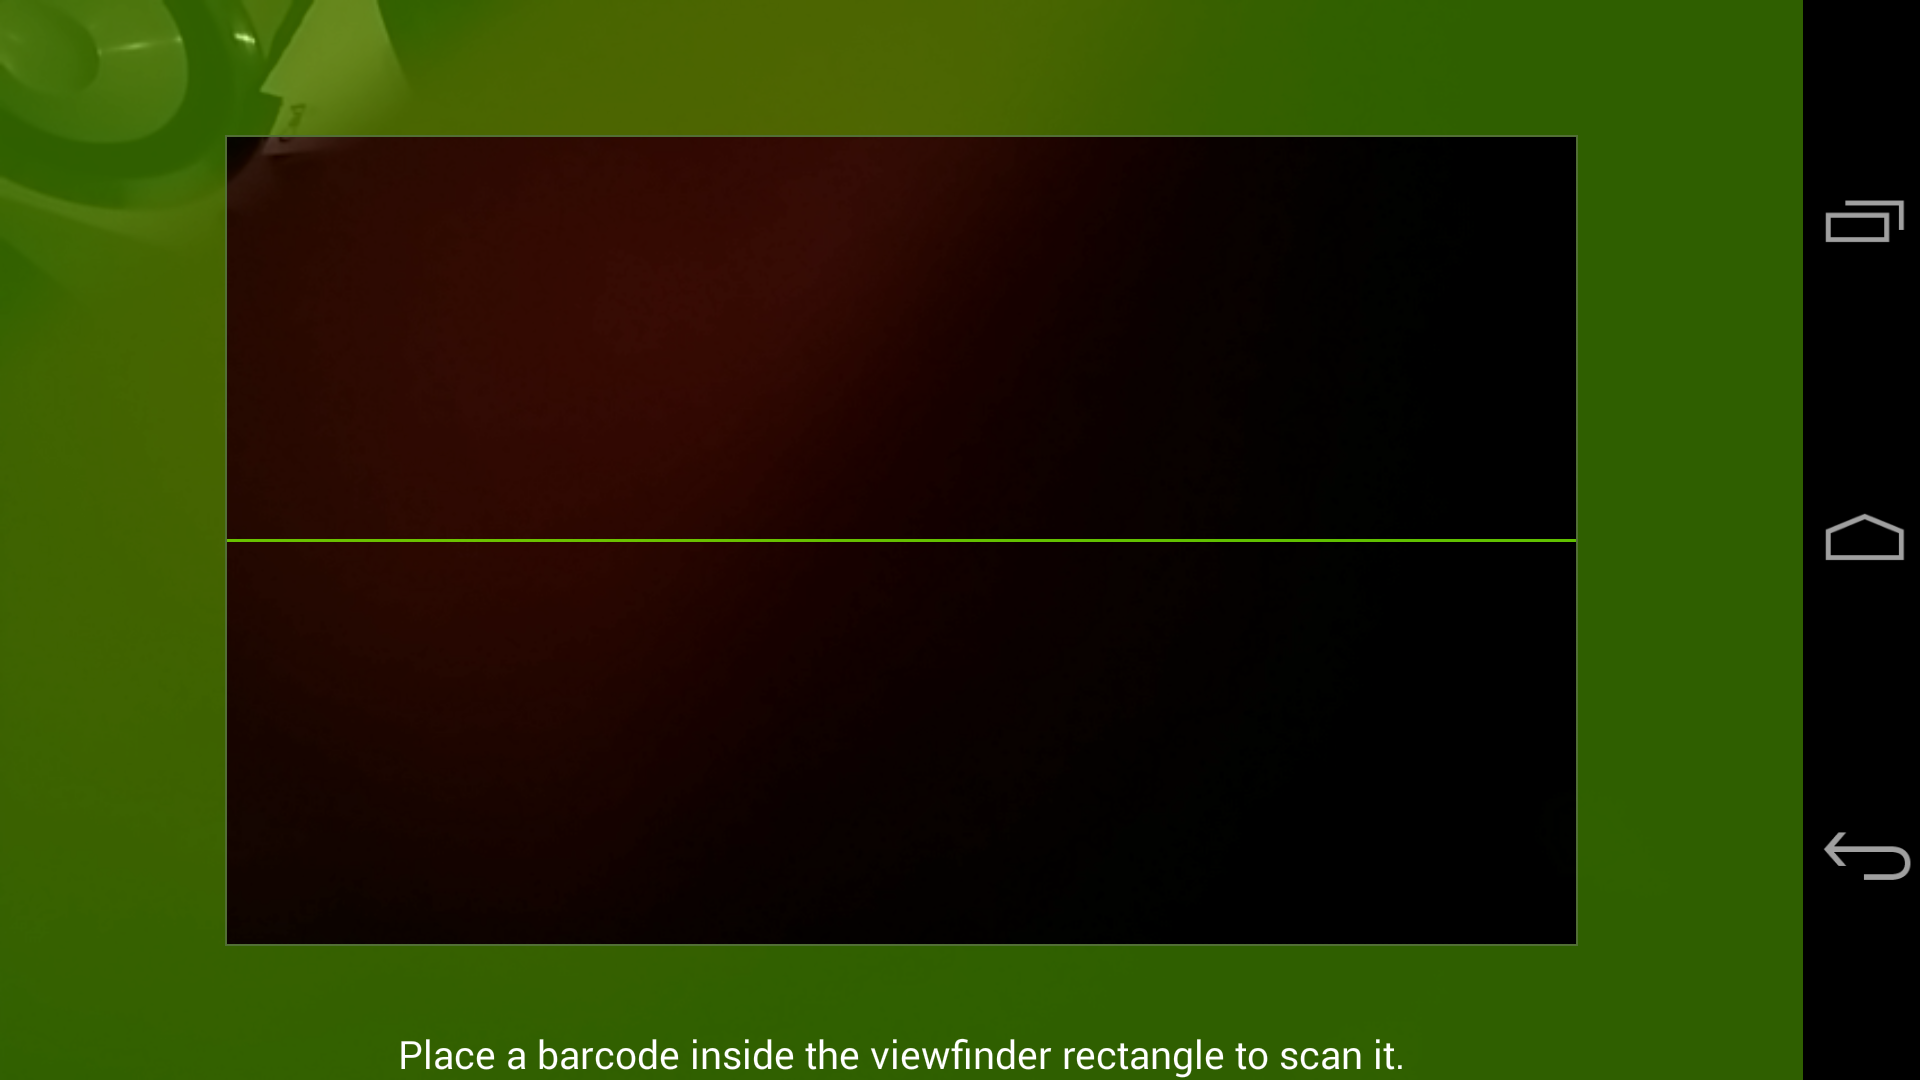
\includegraphics[width=\textwidth]{../screenshots/Screenshot_2013-12-01-20-51-38.png}
\caption{Receiving a DH key exchange via QR codes. The devices switch roles after detecting the initiator.}
\end{subfigure}
\caption{The prototype in use.}
\label{figui}
\end{figure}


\bibliographystyle{plain}
\bibliography{../references/references.bib}

\end{document}

% vim:tw=0:wrap
